% !TEX program = xelatex
\documentclass[11pt,a4paper]{article}

\usepackage[a4paper,margin=24mm,headheight=15pt]{geometry}
\usepackage{fontspec}
\defaultfontfeatures{Ligatures=TeX}
\usepackage{microtype}
\usepackage{amsmath,amssymb}
\usepackage{graphicx}
\usepackage{booktabs}
\usepackage{tabularx}
\usepackage{longtable}
\usepackage{array}
\usepackage{enumitem}
\usepackage{xcolor}
\usepackage{caption}
\usepackage{subcaption}
\usepackage{float}
\usepackage{placeins}
\usepackage{pdflscape}
\usepackage{fancyhdr}
\usepackage{hyperref}

\definecolor{navy}{HTML}{17365D}
\definecolor{blue}{HTML}{2F6690}
\definecolor{teal}{HTML}{2A7F80}
\definecolor{orange}{HTML}{C66A1B}
\definecolor{lightblue}{HTML}{EAF2F8}
\definecolor{lightgray}{HTML}{F3F4F6}
\definecolor{darkgray}{HTML}{4B5563}

\hypersetup{
  colorlinks=true,
  linkcolor=navy,
  urlcolor=blue,
  citecolor=teal,
  pdftitle={Lightcone Regeneration with Neural Operators},
  pdfauthor={Haris}
}

\pagestyle{fancy}
\fancyhf{}
\lhead{\small Neural-Operator Lightcone Regeneration}
\rhead{\small Research Report}
\cfoot{\thepage}
\fancypagestyle{plain}{
  \fancyhf{}
  \lhead{\small Neural-Operator Lightcone Regeneration}
  \rhead{\small Research Report}
  \cfoot{\thepage}
}

\setlength{\parindent}{0pt}
\setlength{\parskip}{0.55em}
\setlist[itemize]{leftmargin=1.4em,itemsep=0.25em,topsep=0.25em}
\setlist[enumerate]{leftmargin=1.6em,itemsep=0.25em,topsep=0.25em}
\captionsetup{font=small,labelfont=bf}
\renewcommand{\arraystretch}{1.18}

\graphicspath{
  {../findings/figures/ufno-detailed_20260606-234954_job3966888/}
  {../findings/figures/sirenfno-spectral-bias_20260621/}
  {../../../_attachments/}
}

\newcommand{\xhi}{x_{\mathrm{HI}}}
\newcommand{\xhii}{x_{\mathrm{HII}}}
\newcommand{\zre}{z_{\mathrm{re}}}
\newcommand{\Ltwo}{L^2}
\newcommand{\Hone}{H^1}
\newcommand{\code}[1]{\texttt{#1}}
\newcommand{\milestone}[1]{\textcolor{navy}{\textbf{#1}}}

\begin{document}

\begin{titlepage}
  \centering
  \vspace*{20mm}
  {\sffamily\color{navy}\Large Master's Thesis Research Report\par}
  \vspace{8mm}
  {\Huge\bfseries Lightcone Regeneration\\[2mm]
  with Neural Operators\par}
  \vspace{7mm}
  {\Large Reconstructing 21cmFAST neutral-fraction lightcones from ground-truth density fields\par}
  \vspace{18mm}
  \rule{0.82\textwidth}{0.8pt}
  \vspace{12mm}

  \begin{minipage}{0.82\textwidth}
  \large
  This report consolidates the planning and experimental findings for a
  field-regeneration pipeline that maps matter-density lightcones and their
  simulation parameters to neutral-hydrogen-fraction lightcones. It follows
  the construction and diagnosis of the 3-D Fourier neural-operator models
  and the current shift toward smooth targets and information-preserving
  line-of-sight sampling.
  \end{minipage}

  \vfill
  {\Large Haris\par}
  \vspace{3mm}
  {\large 16 July 2026\par}
  \vspace{12mm}
  {\small Source: thesis wiki planning and findings notes; figures reproduced
  from the associated experiment artifacts.\par}
\end{titlepage}

\pagenumbering{roman}
\tableofcontents
\clearpage
\listoffigures
\clearpage
\pagenumbering{arabic}

\begin{abstract}
This work studies the regeneration map
\(\delta_m(\mathbf{x},z)\mapsto\xhi(\mathbf{x},z)\). First, density alone is
insufficient: broadcasting the eleven sampled cosmological and astrophysical
parameters reduced validation \(\Ltwo\) from approximately \(0.20\) to
\(0.06\). Second, representation matters: a U-FNO with a local real-space
convolutional path reduced the converged pure-FNO floor from
\((\Ltwo,\Hone)=(0.056,11.36)\) to \((0.0418,8.27)\).

Subsequent work localized the remaining error to ionization fronts. More
spectral modes, stronger \(\Hone\) weighting, alternate normalization, and a
larger line-of-sight receptive field did not break the U-FNO floor. A new
mode-weight diagnostic directly measured rapid low-frequency collapse in
standard FNO/U-FNO kernels. SirenFNO prevented that collapse and improved on a
plain FNO, but remained behind U-FNO because it lacked the latter's local
convolutional path. A windowed Local-FNO also failed to sharpen fronts: after
additional training its transition width remained \(18.5\) Mpc versus
\(13.9\) Mpc for U-FNO in the same diagnostic, while both exhibited a common
``hedging'' bias in nearly ionized voxels.

The current interpretation is therefore broader than spectral bias alone.
The discontinuous target and the coarse low-redshift sampling of the cached
lightcone both impose structural limits. The active programme now attacks
these limits directly: learn a smooth fitted \(\zre(x,y)\) map and reconstruct
\(\xhi\) by thresholding, and replace the uniform-redshift cache with a warped
line-of-sight grid concentrated where ionization changes. The aim is a
faithful regenerated lightcone with correct global timing, morphology,
ionized interiors, and sharp transition fronts.
\end{abstract}

\section{Scope, source material, and organizing principle}

This document is a synthesis rather than a literal concatenation. Repeated
implementation notes were merged, code fragments were reduced to the parts
that affect the scientific argument, and results supersede earlier plans where
the two conflict. The report preserves the chronology because the sequence of
failed and successful interventions is itself the main evidence for the
current diagnosis.

\section{The neural-operator regeneration programme}

\subsection{Task definition}

The target is a full field-to-field regeneration:
\begin{equation}
\mathcal{G}:\;(\delta_m(\mathbf{x},z),\theta)
\longmapsto \xhi(\mathbf{x},z),
\end{equation}
where the density lightcone and the global simulation parameters are treated
as ground-truth inputs. The objective is to reproduce the corresponding
neutral-fraction lightcone generated by 21cmFAST.

The original architecture plan anticipated two facts later confirmed by
experiment:
astrophysical parameters must be supplied to the operator, and a U-shaped
operator is likely to outperform a pure FNO on sharp ionization fronts. It
also established the evaluation axes that matter for regeneration: voxel
accuracy, gradient fidelity, global neutral-fraction history, bubble
morphology, power spectra, cross-correlation, and front sharpness.

\subsection{The first 21cmFAST-to-FNO interface}

The short May meeting note asked for simulation data, approximate-symmetry
tests, and alternative encoders. The associated implementation brief made the
immediate task concrete: read 21cmFAST lightcones, feed the matter density into
an FNO, and predict \(\xhi\).

The resulting pipeline separated simulator and learning environments and
introduced six practices that remained important throughout the later
campaign:
\begin{itemize}
  \item a manifest of lightcone files and their geometry;
  \item simulation-level train/validation/test splits, preventing chunks from
  the same lightcone leaking across splits;
  \item training-only normalization statistics;
  \item full transverse planes with line-of-sight chunks;
  \item checkpoints that store model, normalization, split, and configuration
  metadata together; and
  \item overlapping prediction chunks blended with a Hann window.
\end{itemize}

The first pipeline used relative \(\Ltwo\) and small chunks as a smoke-test
design. The production work later moved to full \(140\times140\times256\)
cubes and absolute \(\Ltwo+\Hone\), because relative norms are ill-conditioned
for all-ionized target regions.

\section{The main 3-D FNO experimental campaign}

\subsection{Production problem and infrastructure}

The production map was
\begin{equation}
\mathcal{G}:\delta_m(\mathbf{x},z)\longmapsto\xhi(\mathbf{x},z)
\end{equation}
over \(6600\) 21cmFAST lightcones of shape
\(140\times140\times256\), spanning \(z=5\) to \(25\). Each input eventually
contained thirteen channels: density divided by ten, \(1/(1+z)\), and eleven
z-scored cosmological and astrophysical parameters broadcast over the volume.

The training objective was
\begin{equation}
\mathcal{L}
=0.5\,\mathcal{L}_{\Ltwo}^{\mathrm{abs}}
+0.5\,\mathcal{L}_{\Hone}^{\mathrm{abs}},
\end{equation}
with Adam, cosine annealing, and a per-rank batch size of one on four H200
GPUs. A precomputed compressed cube cache, direct compressed-chunk copying,
local NVMe staging, and distributed data parallelism reduced iteration time
enough to make the ablation campaign practical.

\subsection{Seven acts of diagnosis}

\begin{table}[H]
\centering
\caption{The central ablation sequence. Validation numbers are the reported
best or converged values for each configuration.}
\small
\begin{tabularx}{\textwidth}{@{}XrrX@{}}
\toprule
Configuration & val \(\Ltwo\) & val \(\Hone\) & Interpretation \\
\midrule
Density only & \(0.20\) & \(17.85\) & Degenerate near-constant predictor. \\
+ eleven parameters & \(0.06\) & \(11.5\) & Timing and morphology become learnable. \\
Modes \(16\to24\) & \(0.06\) & \(11.5\) & More global spectral capacity is unused. \\
+ BCE regularizer, 100 epochs & \(0.0561\) & \(11.36\) & Same asymptote; hedging not fixed by BCE. \\
U-FNO + synchronized BN & \(\mathbf{0.0418}\) & \(\mathbf{8.27}\) &
Local real-space path decisively lowers the floor. \\
More LOS modes + GroupNorm + stronger \(\Hone\) & \(0.0424\) & \(8.36\) &
Cheap tuning knobs do not improve the floor. \\
Anisotropic LOS U-Net stride & \(0.0438\) & \(8.45\) &
Larger LOS receptive field is not the bottleneck. \\
\bottomrule
\end{tabularx}
\end{table}

\subsubsection{Act 1: density alone is not identifiable}

Without astrophysical parameters the model converged to a marginally optimal
constant prediction. Lightcones with similar density structure can have very
different reionization histories, so the mapping is not identifiable from the
input field alone. This failure was not an optimization problem; it was a
missing-information problem.

\subsubsection{Act 2: conditioning is the first breakthrough}

Broadcasting the eleven sampled parameters reduced validation \(\Ltwo\) by
about \(61\%\) at the first epoch relative to the density-only run. The model
immediately learned cone-dependent timing and placed bubbles in the correct
regions. The remaining error shifted to the partially ionized transition,
where the prediction used intermediate values rather than committing to sharp
zero-one interiors.

\subsubsection{Acts 3--4: capacity and loss changes do not remove the floor}

Increasing the retained modes from \(16^3\) to \(24^3\) produced overlapping
training curves. A BCE term also failed to change the converged solution. The
early BCE run looked worse on the hardest low-redshift slices because it made
confident errors, but after \(100\) epochs both objectives reached essentially
the same pure-FNO floor:
\begin{equation}
\boxed{\mathrm{val}\ \Ltwo=0.0561,\qquad
\mathrm{val}\ \Hone=11.36.}
\end{equation}

\subsubsection{Act 5: the U-FNO local path is decisive}

The U-FNO interleaves global spectral blocks with mini 3-D U-Net branches.
With the same inputs, modes, and loss, it reached the pure-FNO asymptote in
three epochs and converged after thirty epochs to
\begin{equation}
\boxed{\mathrm{val}\ \Ltwo=0.0418,\qquad
\mathrm{val}\ \Hone=8.27,}
\end{equation}
with test \(\Ltwo=0.0408\). This is a \(25\)--\(29\%\) improvement across the
main metrics.

The run also exposed a distributed-training failure mode. Ordinary
\code{BatchNorm3d} buffers diverged across ranks at batch size one, producing
unstable validation behavior. Converting the network to synchronized batch
normalization before the DDP wrapper removed the instability. This result is
methodologically important because the apparent architecture failure was
actually inconsistent state in the normalization buffers.

\begin{figure}[p]
\centering
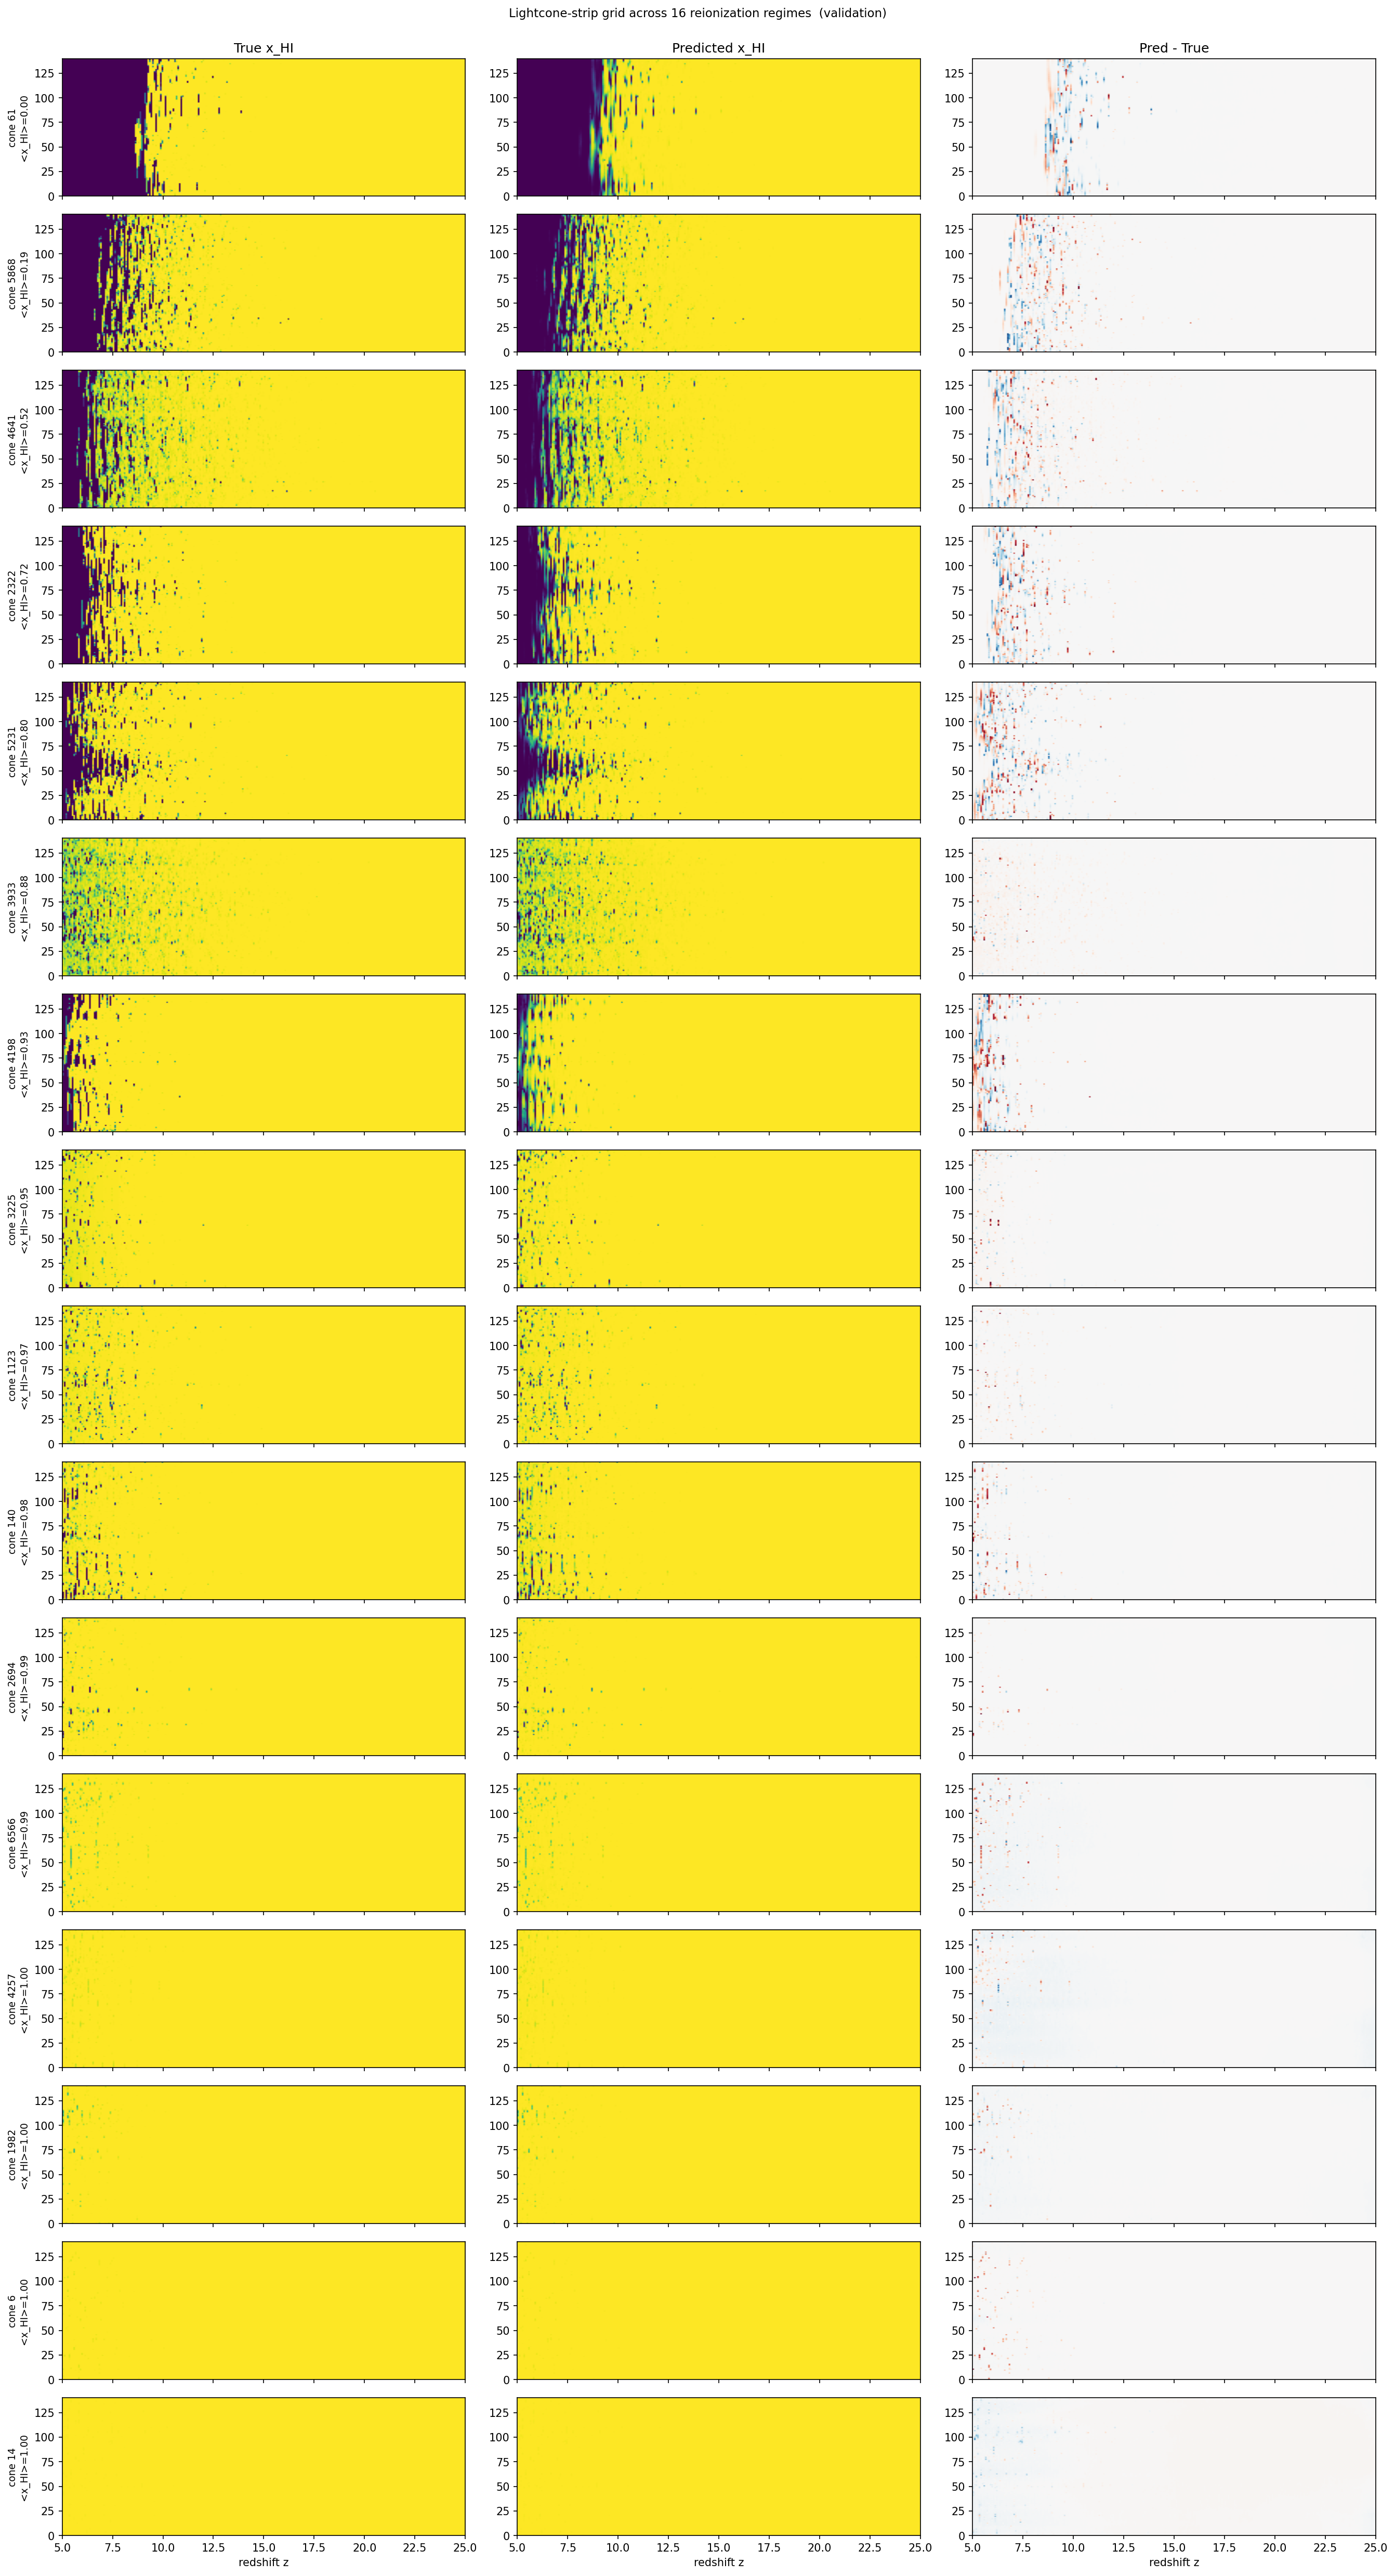
\includegraphics[height=0.82\textheight]{lightcone_grid_3d_validation.png}
\caption{Validation summary for sixteen U-FNO lightcones spanning heavily
reionized to fully neutral cases. Residuals are concentrated in the transition
regions rather than in the saturated parts of the lightcone.}
\label{fig:ufno-grid}
\end{figure}

\begin{figure}[p]
\centering
\begin{subfigure}[t]{0.48\textwidth}
\centering
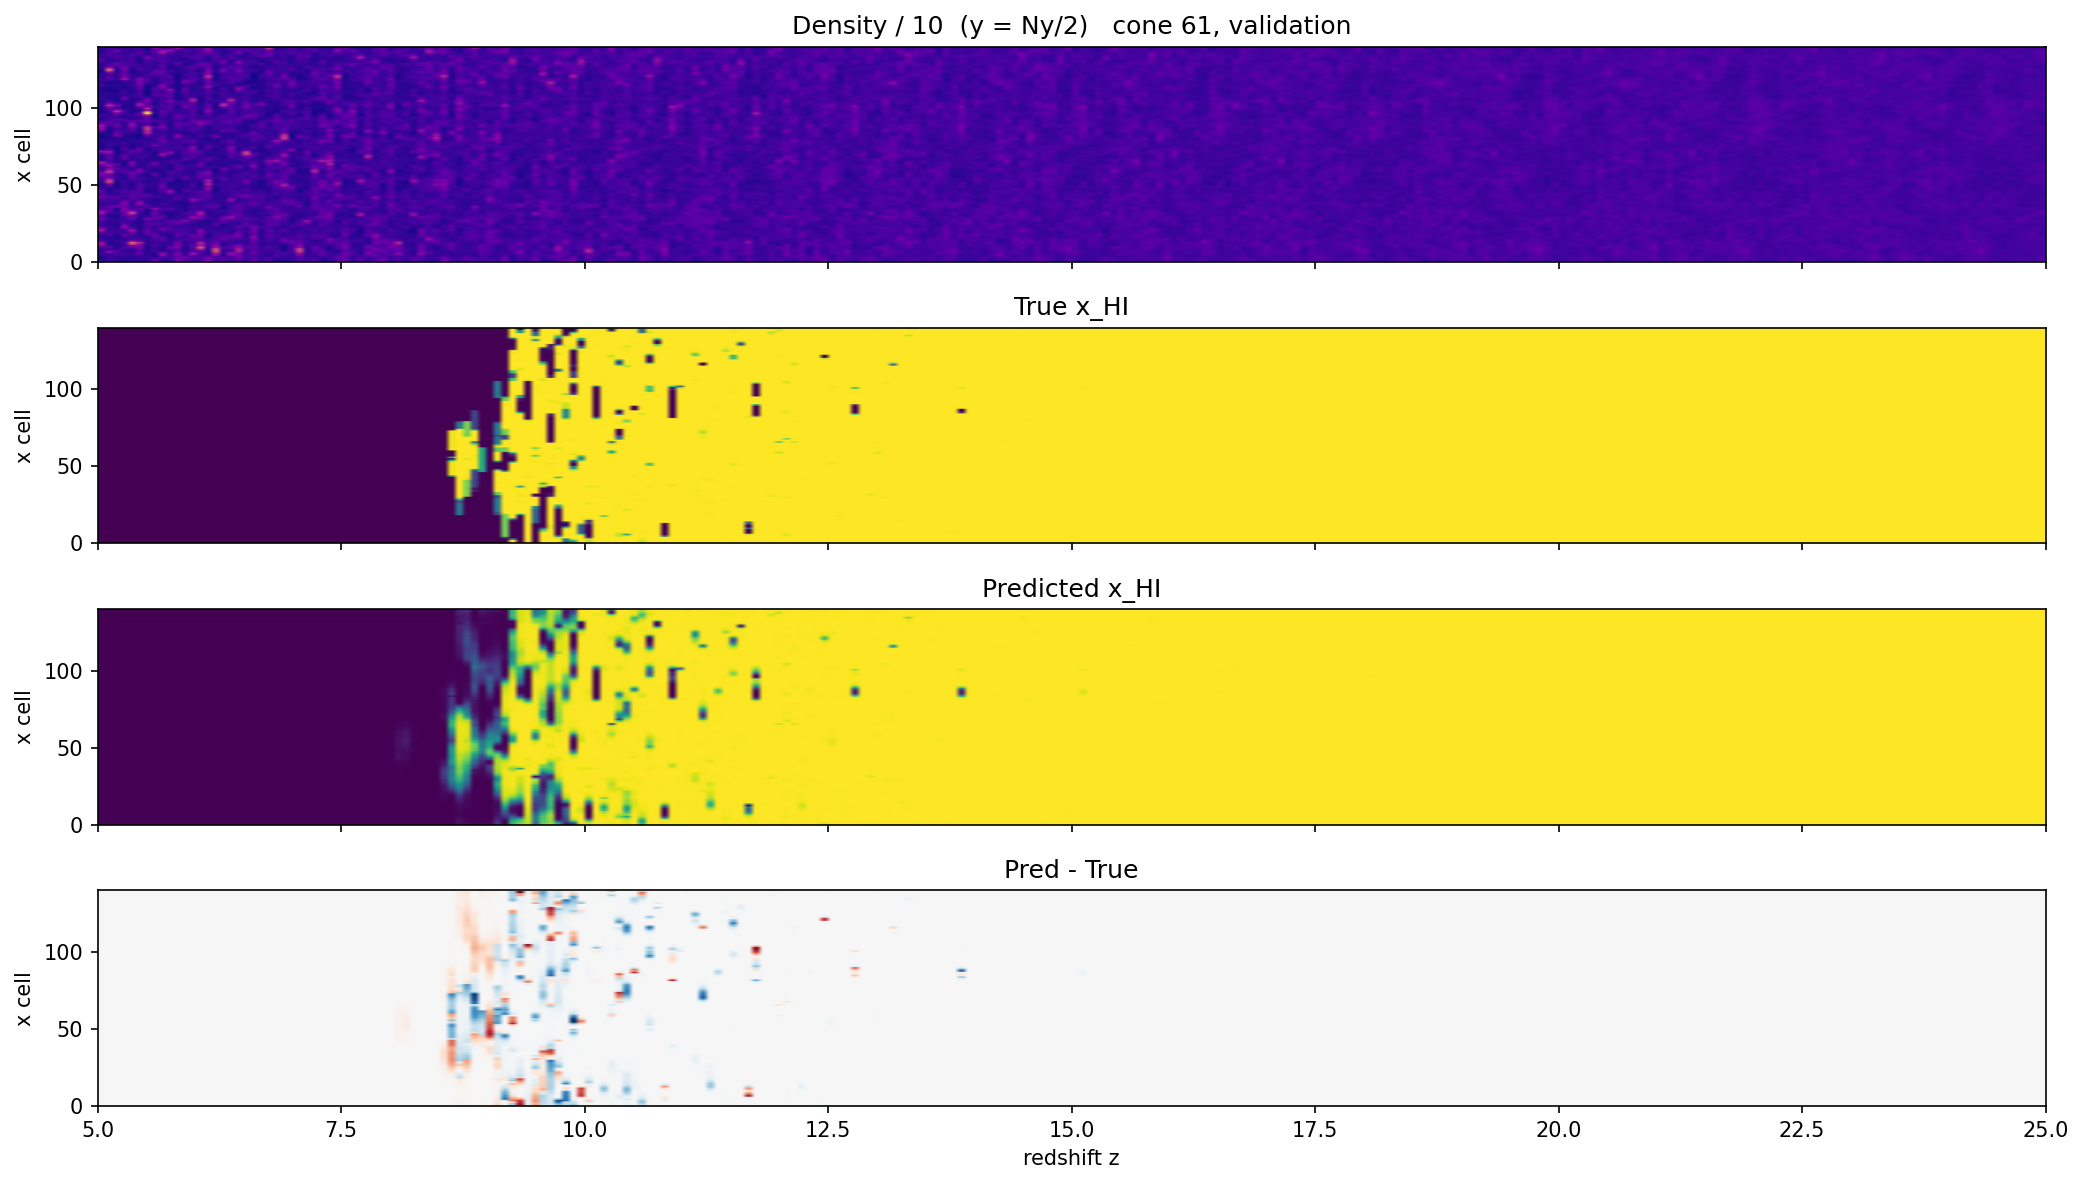
\includegraphics[width=\linewidth]{lightcone_3d_validation_cone61.png}
\caption{Cone 61: heavily reionized.}
\end{subfigure}\hfill
\begin{subfigure}[t]{0.48\textwidth}
\centering
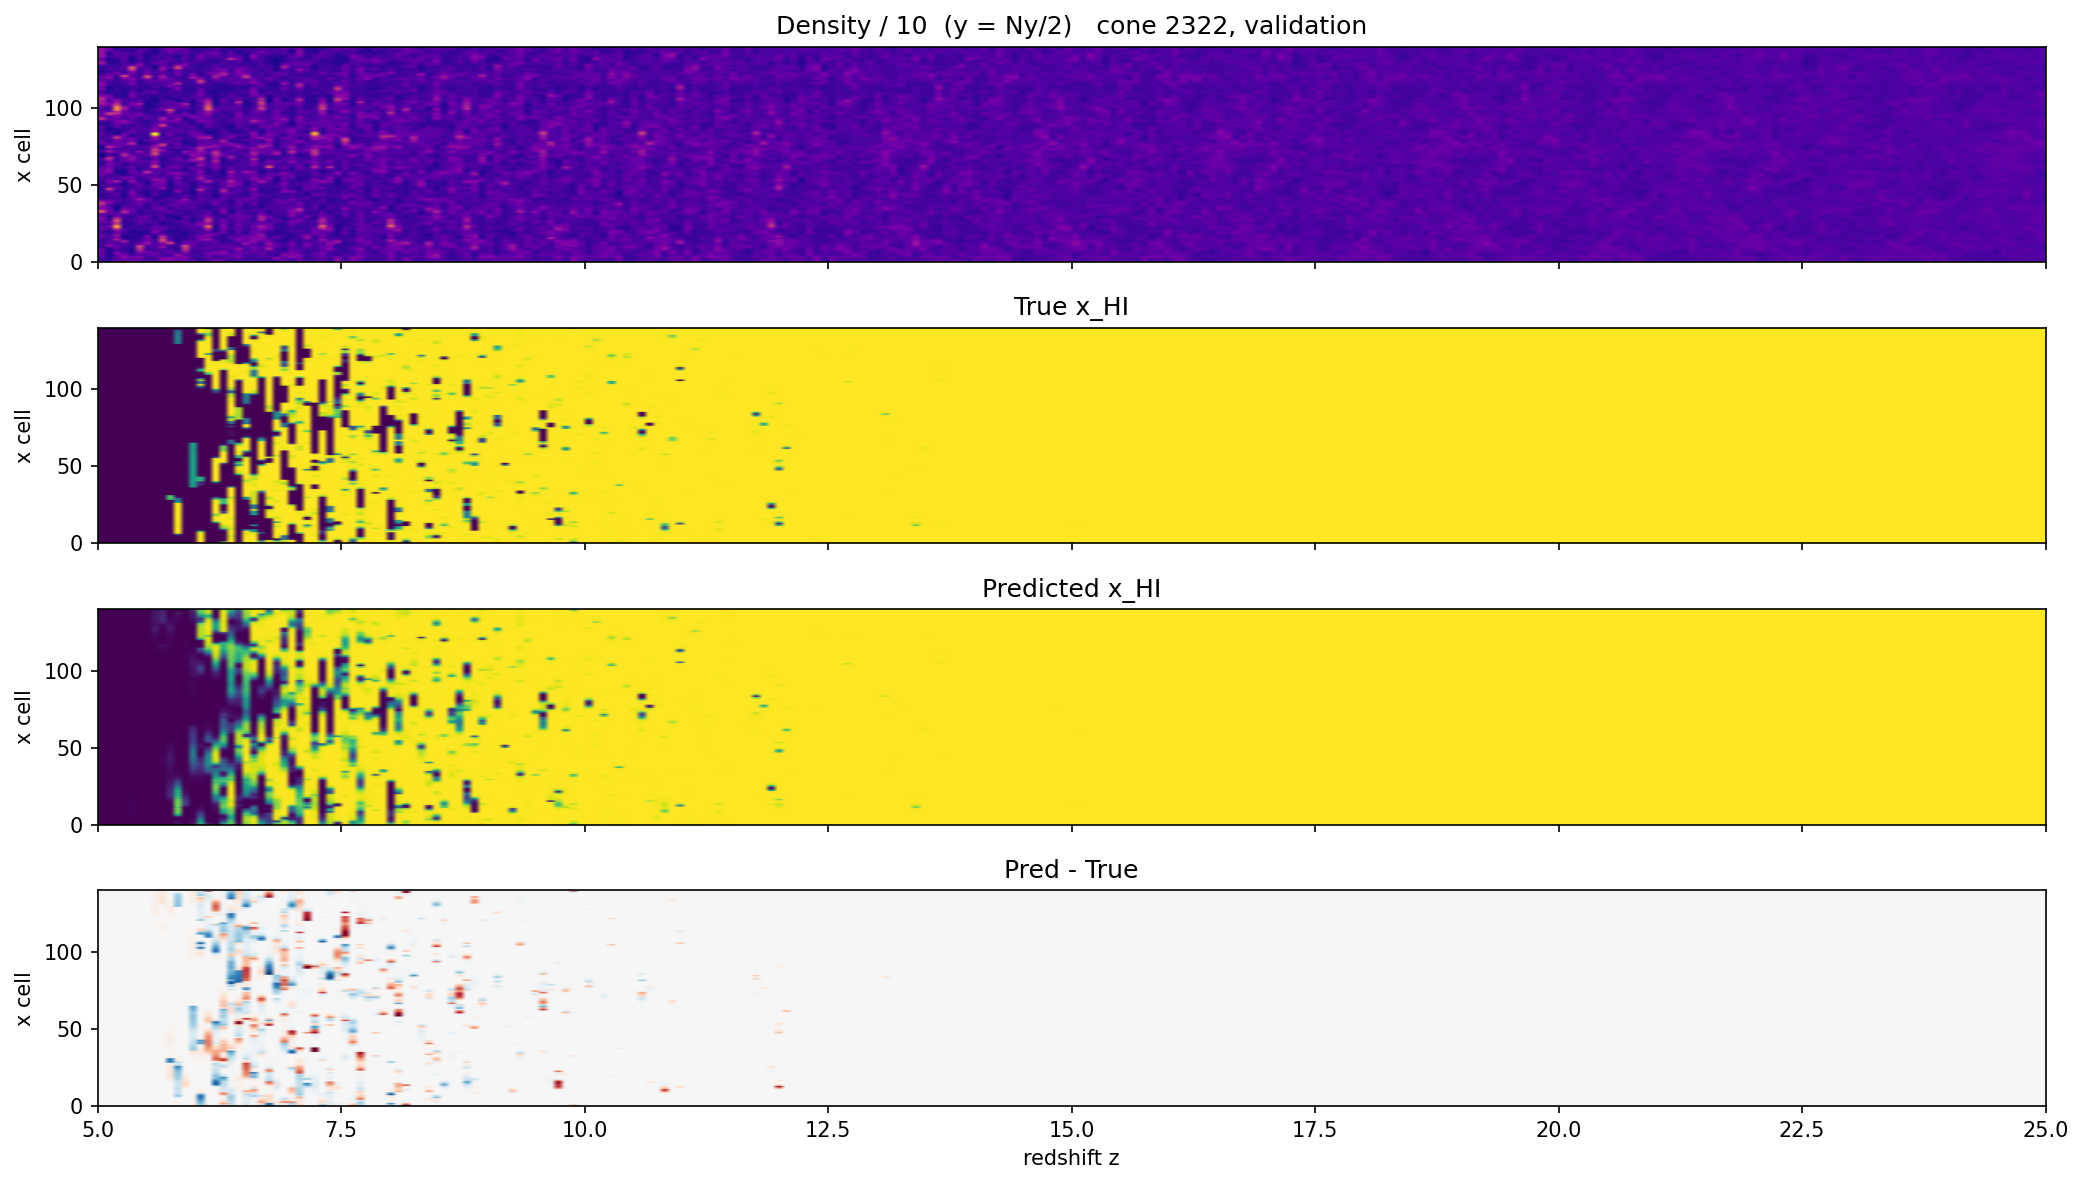
\includegraphics[width=\linewidth]{lightcone_3d_validation_cone2322.png}
\caption{Cone 2322: patchy transition.}
\end{subfigure}

\vspace{4mm}
\begin{subfigure}[t]{0.48\textwidth}
\centering
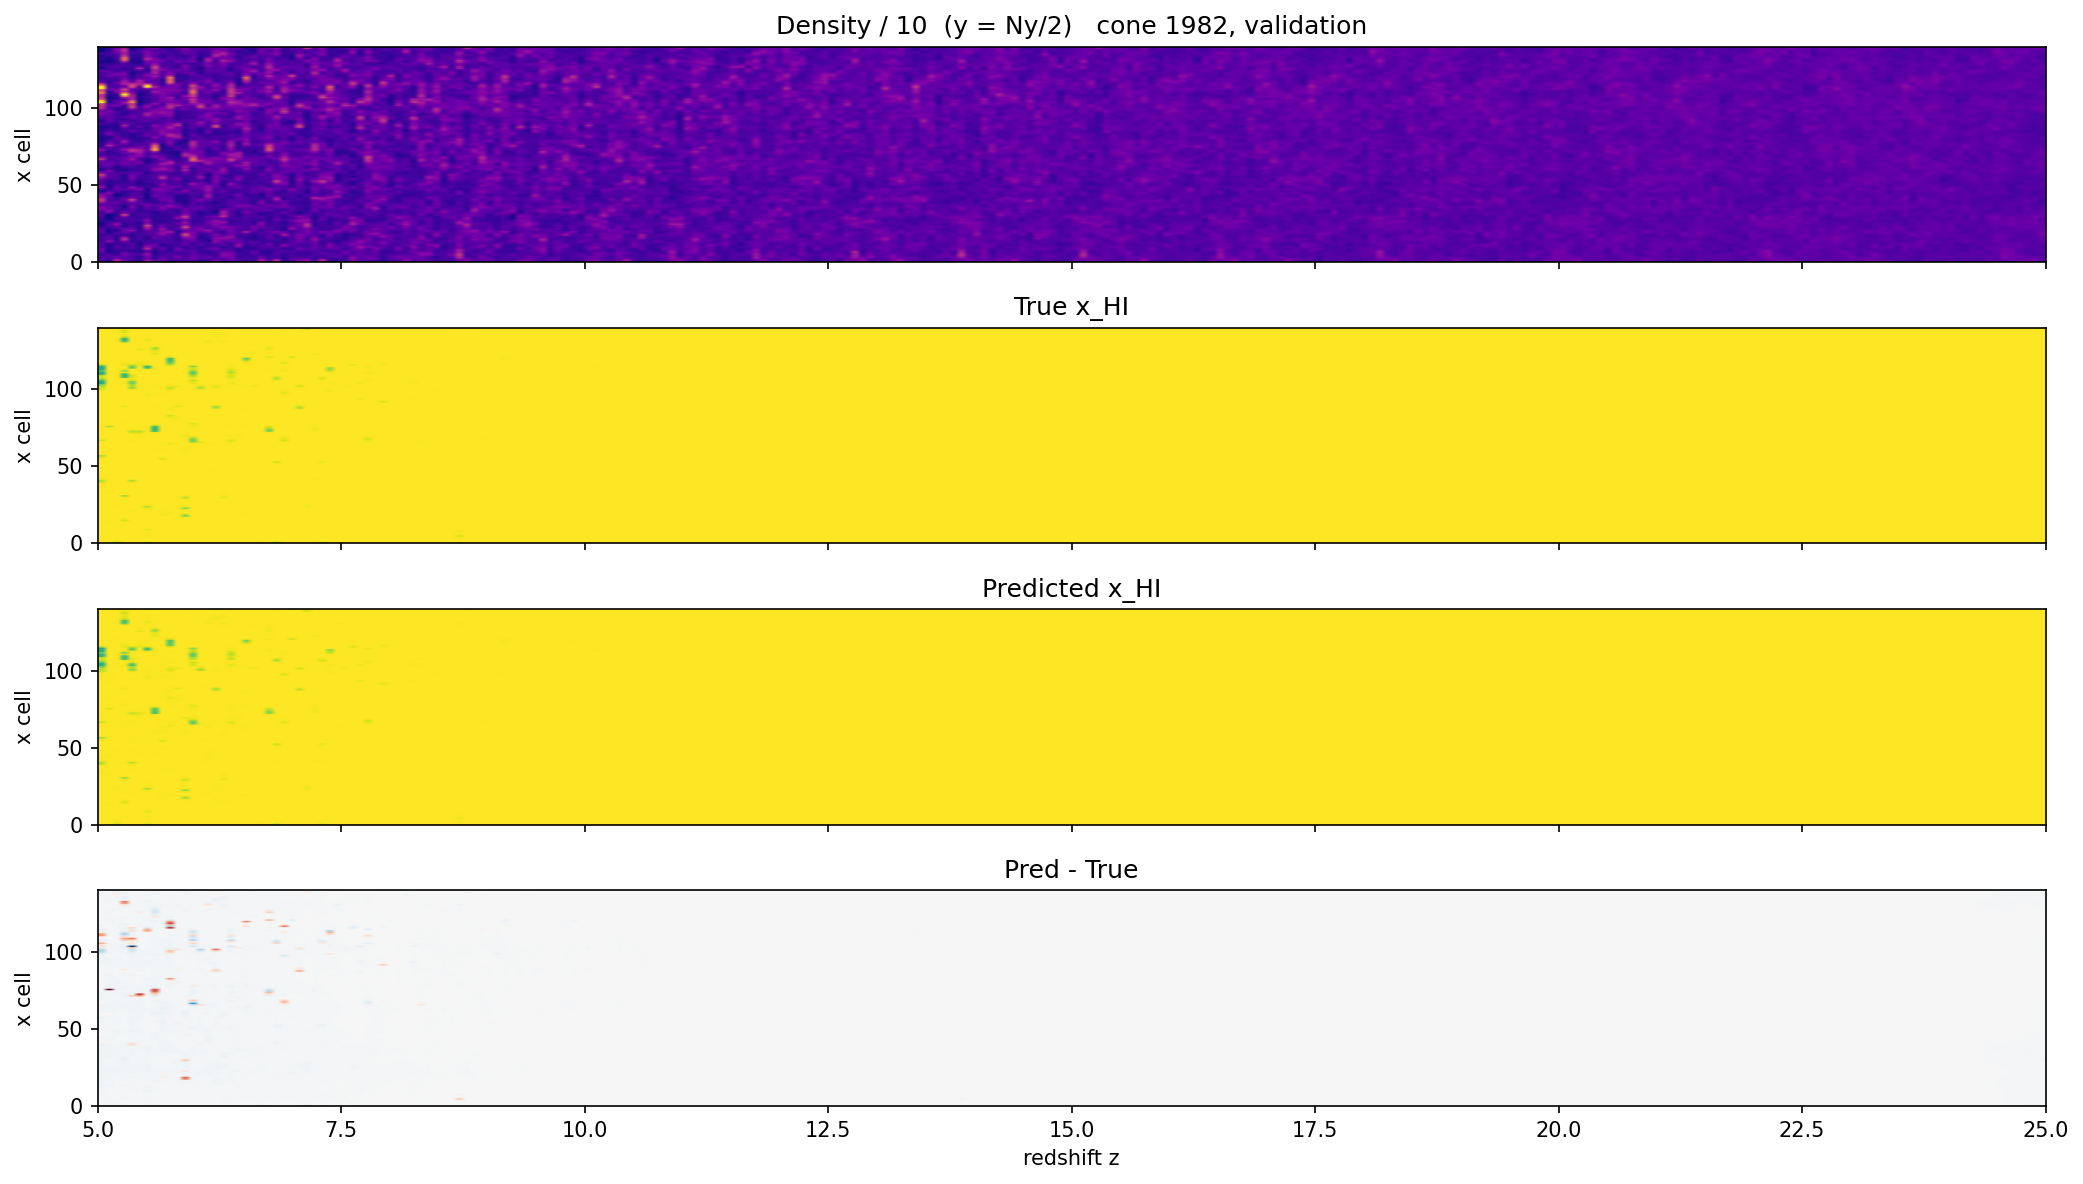
\includegraphics[width=\linewidth]{lightcone_3d_validation_cone1982.png}
\caption{Cone 1982: fully neutral.}
\end{subfigure}
\caption{Three diagnostic U-FNO cones. The model captures global timing and
morphology; the remaining discrepancies trace bubble boundaries.}
\label{fig:ufno-cones}
\end{figure}
\FloatBarrier

\subsubsection{Acts 6--7: the U-FNO floor survives internal tuning}

Doubling the line-of-sight spectral bandwidth, replacing synchronized batch
normalization with GroupNorm, and increasing the \(\Hone\) loss weight did not
improve the benchmark. An anisotropic U-Net with a larger LOS bottleneck
receptive field started from a better first epoch but converged to the same
neighborhood. These nulls rule out a simple explanation based on missing LOS
context inside the local path.

The defensible interpretation of the repeated mode-count null is precise:
\code{n\_modes} controls learned global Fourier communication, not the output
bandwidth of the entire nonlinear network. Increasing that communication
bandwidth did not improve the solution; it does not follow that all
high-frequency output was hard-truncated.

\subsection{What the campaign established}

The June campaign separated two necessary ingredients:
\begin{itemize}
  \item \milestone{Input information}: the eleven parameters are required to
  identify the reionization history.
  \item \milestone{Inductive bias}: a local real-space path represents sharp
  structures better than adding capacity to the same global Fourier basis.
\end{itemize}

The remaining residual is highly nonuniform in redshift. For a representative
test cone the per-voxel MSE was about \(0.085\) at \(z=5\), but only
\(2\times10^{-4}\) to \(5\times10^{-4}\) in fully neutral high-redshift
slices. Whole-volume metrics therefore conceal the physical location of the
problem: ionization fronts.

\section{Residual refinement and direct spectral diagnosis}

\subsection{The Siren3D residual plan}

The first response to the U-FNO floor was a narrow residual experiment rather
than a wholesale replacement. A frozen U-FNO supplies a prediction and latent
context at each coordinate, while a sinusoidal MLP predicts a gated logit
correction:
\begin{equation}
\widehat{\xhi}(\mathbf{r})
=\sigma\!\left[
\operatorname{logit}\widehat{\xhi}_{\mathrm{UFNO}}(\mathbf{r})
+\alpha f_{\mathrm{SIREN}}(\mathbf{r},c(\mathbf{r}))
\right],
\end{equation}
where \(\alpha\) begins at zero. Boundary voxels are oversampled, but a uniform
sample fraction is retained to protect calibration away from fronts. The plan
requires SIREN to beat parameter-matched ReLU, Fourier-feature, and
convolutional residual heads; otherwise any gain cannot be attributed to the
sinusoidal representation.

\subsection{A mode-weight diagnostic turns a hypothesis into a measurement}

Before committing to the residual head, the spectral kernel itself was
instrumented. For every layer and epoch, the per-mode RMS kernel weight was
logged. Three summaries were used:
\begin{itemize}
  \item the weight profile over mode number;
  \item the ratio of outer-quarter to inner-quarter RMS weight; and
  \item the fraction of total weight held by the lowest quarter of modes.
\end{itemize}

At initialization the low-quarter fraction is \(0.25\). In the 32-mode U-FNO,
training moved it to \(0.603\) during epoch zero and \(0.521\) at convergence:
the lowest eight of thirty-two LOS modes held \(52\%\) of the spectral weight.
The 64-mode model showed the same qualitative collapse.

\begin{figure}[p]
\centering
\begin{subfigure}[t]{0.88\textwidth}
\includegraphics[width=\textwidth]{ufno32_z_profiles.png}
\caption{Per-layer U-FNO profiles with 32 LOS modes.}
\end{subfigure}

\vspace{4mm}
\begin{subfigure}[t]{0.72\textwidth}
\includegraphics[width=\textwidth]{ufno32_z_cutoff_ratio.png}
\caption{High-mode to low-mode RMS ratio during training.}
\end{subfigure}
\caption{The U-FNO kernel rapidly learns a low-frequency preference. Extra
modes exist in the parameterization but receive much less weight.}
\label{fig:ufno-bias32}
\end{figure}

\begin{figure}[p]
\centering
\includegraphics[width=0.92\textwidth]{ufno64_z_profiles.png}
\caption{The same learned low-frequency collapse for a U-FNO with 64 LOS
modes. The bias persists when more bandwidth is made available.}
\label{fig:ufno-bias64}
\end{figure}
\FloatBarrier

\subsection{SirenFNO removes the collapse but not the U-FNO advantage}

SirenFNO replaces the independent per-mode kernel table with a SIREN
hypernetwork evaluated over the full Fourier grid. In the implemented
64-mode 3-D model, the low-quarter fraction remained approximately \(0.25\)
throughout training and the cutoff ratio stayed near unity along the Cartesian
axes. The learned spectrum remained flat instead of concentrating on low
modes.

\begin{figure}[p]
\centering
\includegraphics[width=0.95\textwidth]{sirenfno_profiles.png}
\caption{SirenFNO Fourier-weight profiles. Unlike the standard kernel table,
the SIREN-generated kernel remains nearly flat across modes and epochs.}
\label{fig:siren-profiles}
\end{figure}

\begin{figure}[p]
\centering
\begin{subfigure}[t]{0.95\textwidth}
\includegraphics[width=\textwidth]{sirenfno_cutoff_ratio.png}
\caption{Cutoff ratios remain close to one on the coordinate axes.}
\end{subfigure}

\vspace{4mm}
\begin{subfigure}[t]{0.95\textwidth}
\includegraphics[width=\textwidth]{sirenfno_evolution.png}
\caption{Evolution heatmap: no persistent low-mode hot stripe develops.}
\end{subfigure}
\caption{Two views of full-frequency kernel learning in SirenFNO.}
\label{fig:siren-fullfreq}
\end{figure}
\FloatBarrier

The aggregate held-out comparison was:
\begin{table}[H]
\centering
\caption{Held-out performance of the main spectral representations.}
\begin{tabular}{@{}lrrrr@{}}
\toprule
Model & Modes & Epochs & Test \(\Ltwo\) & Test \(\Hone\) \\
\midrule
Plain FNO & \(16^3\) & 100 & \(0.0570\) & \(11.64\) \\
SirenFNO & \(64^3\) & 70 & \(0.0501\) & \(9.82\) \\
U-FNO & \(16^3\) & 100 & \(\mathbf{0.0397}\) & \(\mathbf{7.87}\) \\
\bottomrule
\end{tabular}
\end{table}

Thus SirenFNO improved substantially over the plain FNO but did not beat the
U-FNO. This is not a clean rejection of full-frequency learning because the
tested SirenFNO lacked the U-FNO's real-space convolutional branch. The
controlled next comparison is therefore SirenFNO plus a U-Net path versus
the ordinary U-FNO.

\begin{figure}[p]
\centering
\begin{subfigure}[t]{0.58\textwidth}
\centering
\includegraphics[width=\linewidth,height=0.70\textheight,keepaspectratio]{sirenfno_comparison_test_cone1.png}
\caption{Field-level comparison across representative slices.}
\end{subfigure}\hfill
\begin{subfigure}[t]{0.36\textwidth}
\centering
\includegraphics[width=\linewidth]{sirenfno_scatter_test_cone1.png}
\caption{Voxel parity for test cone 1: \(R^2=0.93\), RMSE \(=0.088\).}
\end{subfigure}
\caption{SirenFNO captures timing and bubble morphology, but its aggregate
error remains above the U-FNO benchmark.}
\label{fig:siren-field}
\end{figure}
\FloatBarrier

\section{The windowed Local-FNO test}

\subsection{Architecture and hypothesis}

The Local-FNO was designed to test whether localizing the Fourier transform
could reproduce the wall sharpness of the U-FNO without using its explicit
real-space convolutional path. The model applies shared 3-D FFT kernels inside
overlapping \(16\times16\times32\) windows, retains
\(6\times6\times12\) local modes, alternates shifted window grids, and uses
square-root Hann analysis and synthesis windows with normalized overlap-add.
Two global FNO blocks operate at a \(35\times35\times64\) bottleneck.

The local and global branches were intended to divide the task:
local windows provide inexpensive high effective frequencies, the global
bottleneck coordinates large bubbles, and U-Net skip connections preserve
high-resolution information. The initial success criterion was better
boundary-band \(\Hone\) and transition width than U-FNO with no more than a
five per cent validation-\(\Ltwo\) regression and no patch seams.

\subsection{First result: a smooth but broader front}

At epoch 20 the Local-FNO had test \(\Ltwo=0.0569\) and
\(\Hone=10.25\), approximately the plain-FNO regime. More importantly, the
front-localized diagnostic directly contradicted the design hypothesis:
\begin{table}[H]
\centering
\caption{Initial boundary-band comparison.}
\begin{tabular}{@{}lrrr@{}}
\toprule
Metric & Truth & U-FNO & Local-FNO, epoch 20 \\
\midrule
10--90\% front width & \(3.6\) Mpc & \(10.7\) Mpc & \(32.2\) Mpc \\
Peak boundary RMSE & -- & \(\sim0.28\) & \(\sim0.32\) \\
Peak gradient error & -- & \(\sim0.16\) & \(\sim0.19\) \\
\bottomrule
\end{tabular}
\end{table}

The overlap-add machinery succeeded in suppressing patch seams, but the
prediction was globally over-smoothed. This suggests that locality alone is
not the mechanism behind the U-FNO gain: a windowed Fourier basis remains a
Fourier basis inside each patch, while the U-FNO supplies a genuinely
Gibbs-free real-space convolutional route.

\begin{figure}[p]
\centering
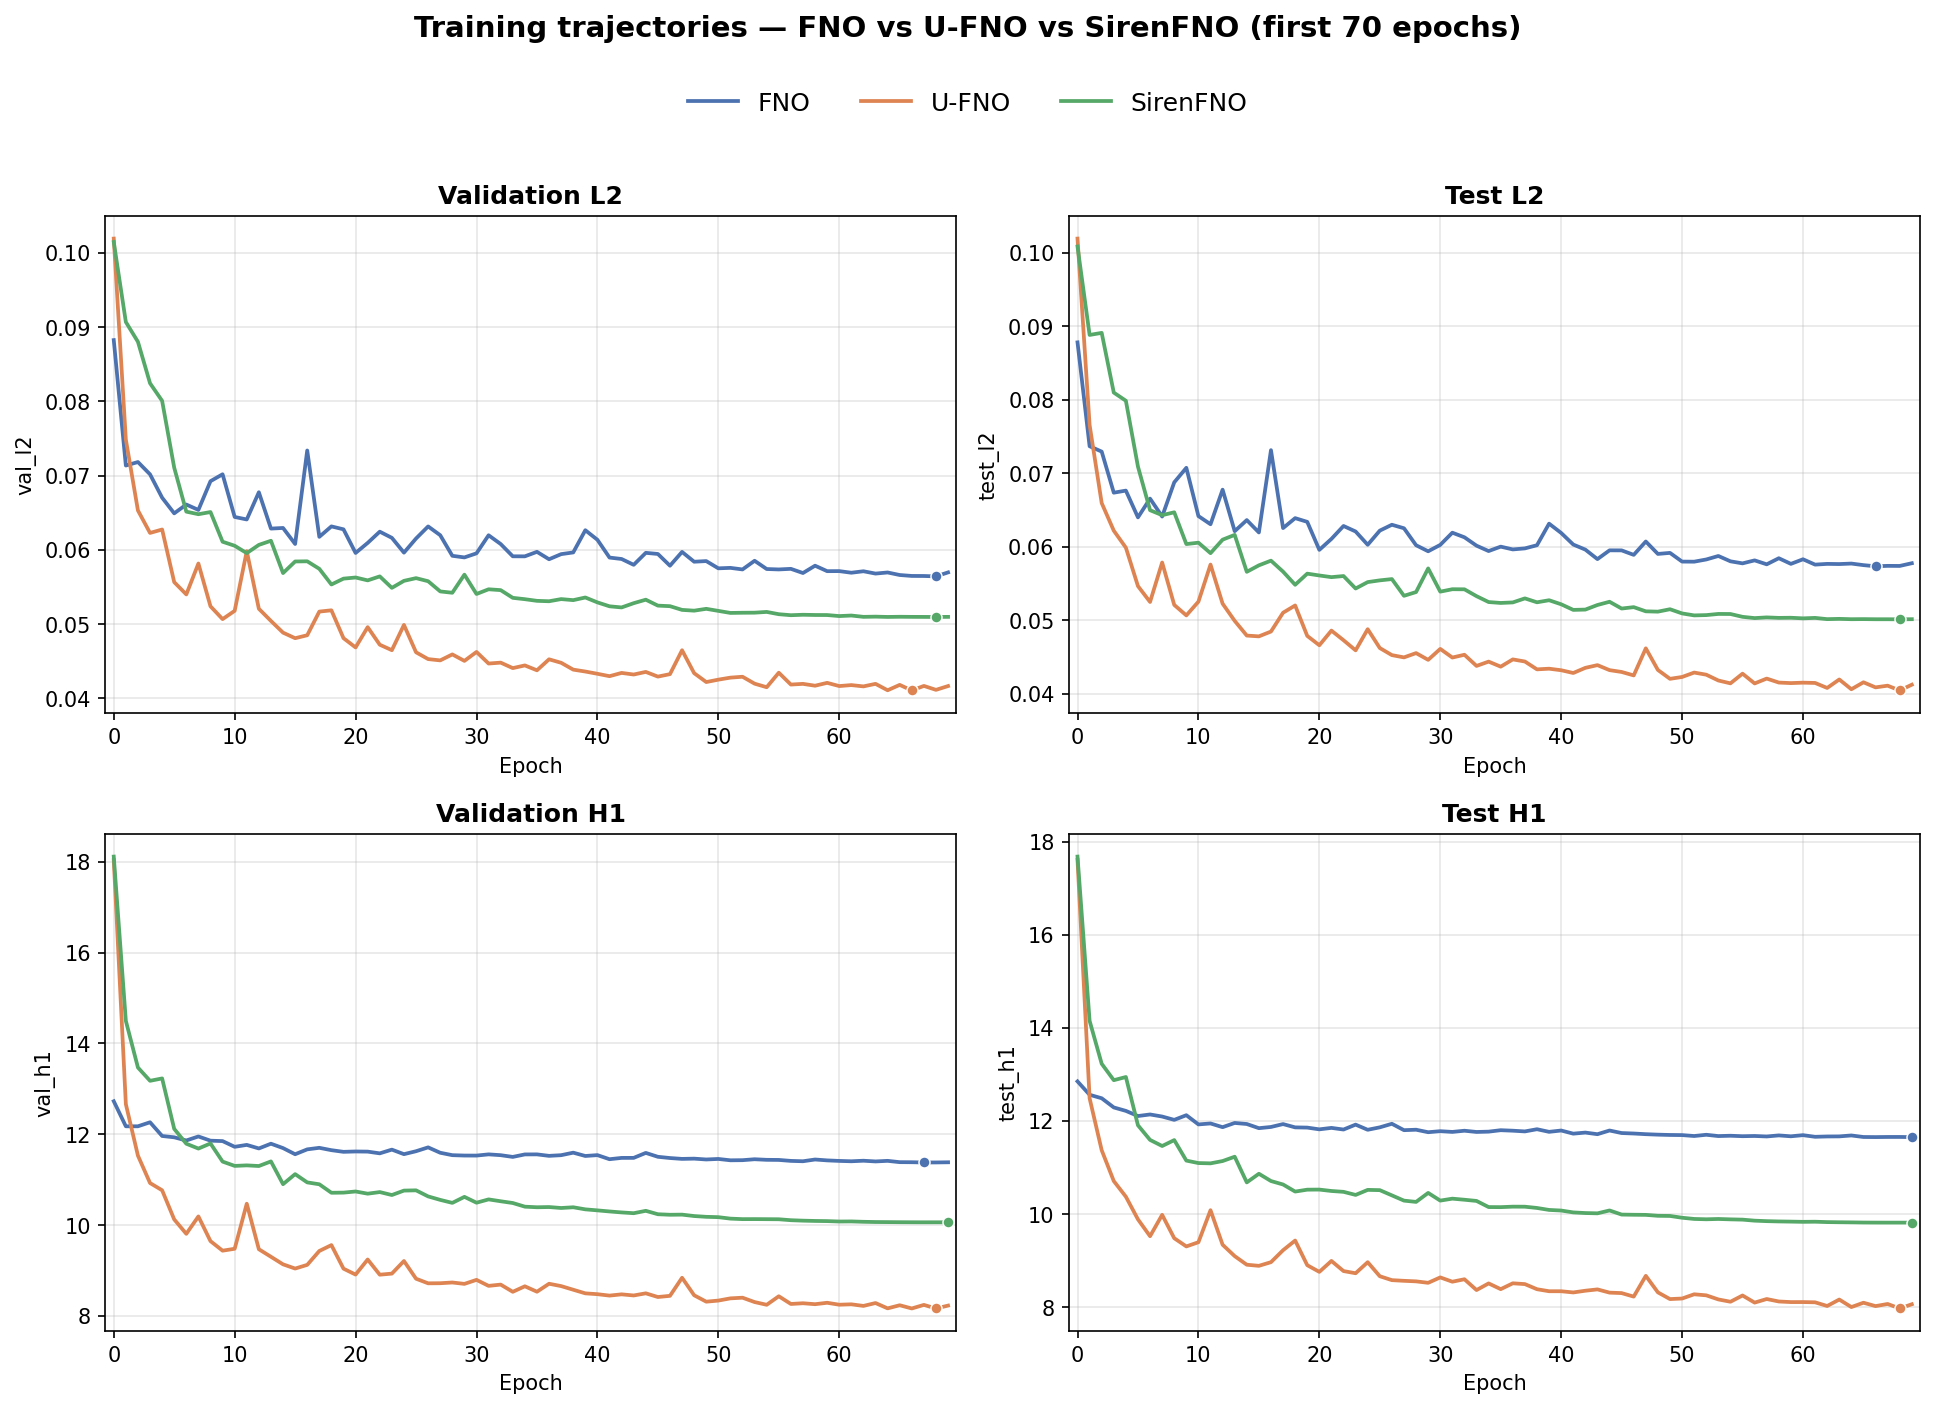
\includegraphics[width=0.96\textwidth]{fno_training_trajectories.png}
\caption{Benchmark training trajectories used to contextualize the
Local-FNO run. The Local-FNO metrics were logged separately and remained
descending at the first reported checkpoint.}
\label{fig:training-trajectories}
\end{figure}

\begin{figure}[p]
\centering
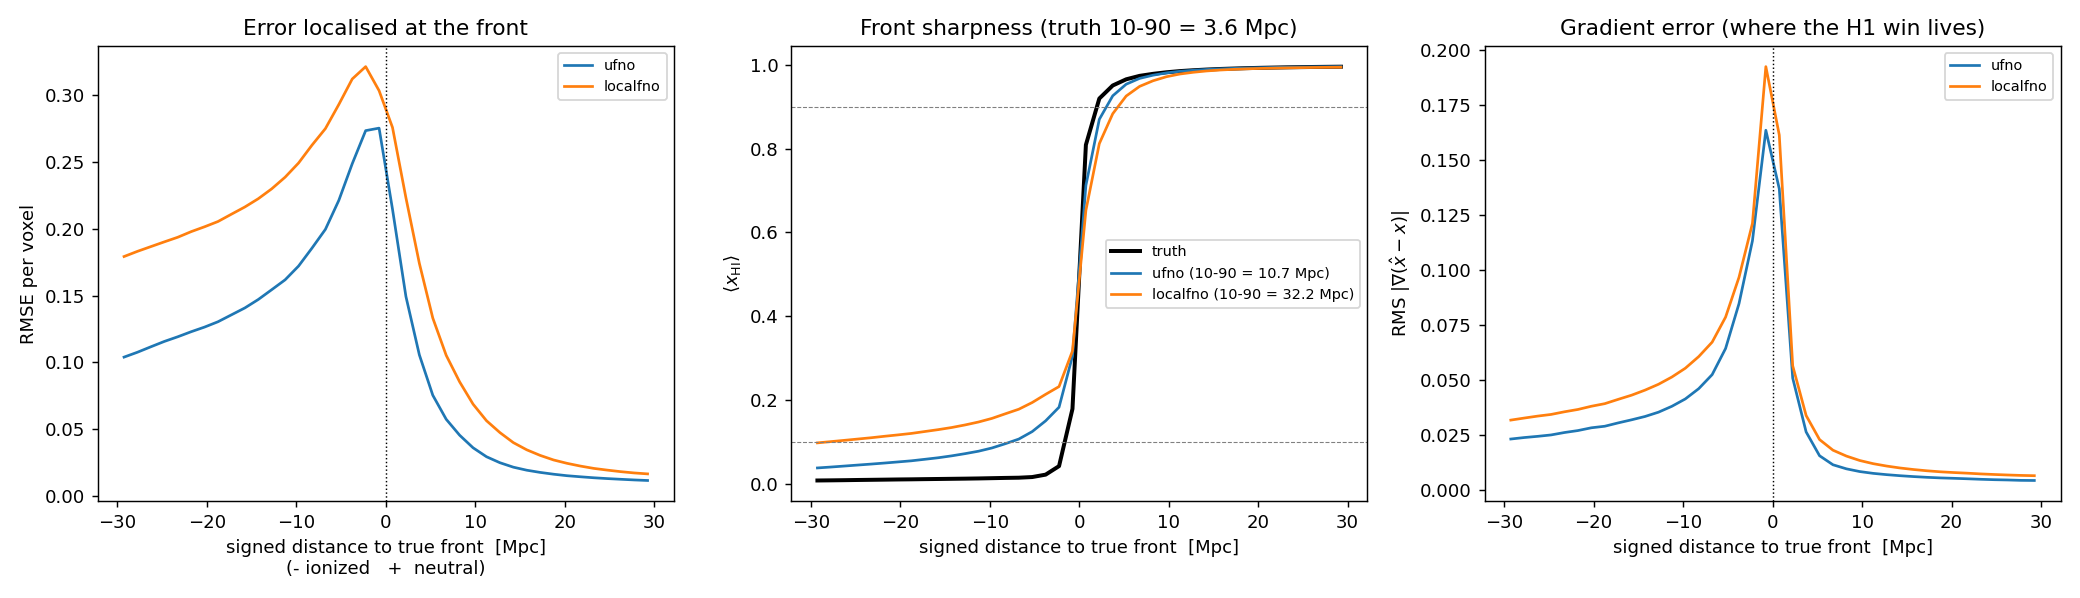
\includegraphics[width=0.98\textwidth]{localfno_boundary_band_overlay.png}
\caption{Boundary-band comparison of U-FNO and the first Local-FNO
checkpoint. The Local-FNO has higher error around the front and a substantially
broader stacked transition profile.}
\label{fig:local-boundary}
\end{figure}
\FloatBarrier

\subsection{Later update: training helps, but the ordering does not flip}

At epoch 38 the within-run front-width comparison improved to \(18.5\) Mpc for
Local-FNO versus \(13.9\) Mpc for U-FNO. The absolute U-FNO number differed
from the earlier diagnostic because the evaluation configuration changed, so
only the within-run comparison is valid. A paired bootstrap still found the
Local-FNO boundary-band \(\Hone\) significantly worse. A one-sided ionized-wall
penalty also failed at the tested training budget.

The new parity diagnostic clarified the common failure. In nearly ionized
voxels with true \(\xhi\) between \(0.02\) and \(0.08\), both models predicted
values that were too high. U-FNO medians were roughly \(0.11\)--\(0.14\);
Local-FNO was worse. The best model therefore still hedges instead of
committing bubble interiors to zero. This observation shifted the diagnosis
from ``insufficient spectral bandwidth'' toward ``a regression target whose
optimal uncertain prediction is intrinsically diffuse.''

\section{Reformulating the target and the data grid}

\subsection{Smooth-target reparameterization}

The new target-side strategy stops asking a smooth regressor to reproduce a
thresholded field directly. Instead, it predicts a smooth latent and applies
the sharp nonlinearity deterministically:
\begin{equation}
\widehat{\xhi}(\mathbf{x},z)
=\mathbb{1}\!\left[z>\widehat{\zre}(\mathbf{x})\right].
\end{equation}
An error in \(\widehat{\zre}\) moves a sharp front; it cannot broaden the front
by averaging zero and one. This matches the generative structure of
excursion-set reionization more closely than direct voxel regression.

Three targets were ranked:
\begin{enumerate}
  \item the reionization-redshift field \(\zre\), preferred for its smoothness
  and direct physical meaning;
  \item a signed distance field to the nearest front, which avoids a monotonic
  ionization assumption; and
  \item the pre-threshold excursion-set latent, the most physically direct but
  the most difficult to expose from 21cmFAST.
\end{enumerate}

The decisive metric remains reconstructed-\(\xhi\) performance, especially
front width, \(P(k)\), cross-correlation, and global history. Good target-space
loss alone is not sufficient because small timing errors can produce large
spatial front displacements.

\subsection{Implemented variant: a fitted 2-D
\texorpdfstring{\(\zre(x,y)\)}{z-re(x,y)} map}

The first implementation avoids rerunning the simulator and avoids the geometry
change associated with a native coeval \(\zre\) box. Each lightcone sightline
is fitted independently, producing a two-dimensional reionization-time map.
Two least-squares definitions are available:
\begin{itemize}
  \item a two-parameter Gompertz front, with the stored target equal to its
  half-neutral redshift; and
  \item the exact least-squares step transition.
\end{itemize}

The model receives \(64\) interpolated density slices as channels, together
with the eleven broadcast parameters, and predicts the 2-D map using an
FNO2d, U-FNO2d, or Local-FNO2d. Undefined pixels are stored as NaN, clamped to
the low-redshift edge for tensor operations, and accompanied by a mask.

The first reconstruction ceiling check is encouraging but exposes a major
class imbalance. Low-redshift and least-squares step crossings reconstruct
global \(\xhi(z)\) with voxel MSE of roughly \(0.008\)--\(0.05\) on the sampled
cones, whereas the high-redshift crossing is poor. However, late-reionizing
cones contain \(79\)--\(99\%\) pixels whose front lies outside the lightcone.
Mask-weighted loss, cone filtering, and the choice between a Gompertz midpoint
and a step target must therefore be resolved by the first training runs.

\subsection{Warping the line-of-sight cache grid}

The target reformulation is complemented by a data-side diagnosis. Native
lightcones contain roughly \(2340\) LOS samples at about \(1.43\) Mpc comoving
spacing. The cube cache downsamples these to \(256\) samples uniformly in
redshift. Because the \(z\)-to-distance conversion is nonlinear, this is
coarsest at low redshift: approximately \(37\) Mpc precisely where the
ionization fronts are active, compared with about \(5\) Mpc in the saturated
high-redshift region.

Any structure erased during caching is unavailable to every downstream model.
The new training-free evaluator therefore performs a native-to-grid-to-native
round trip and measures transition RMSE, sharpness retention, missed fronts,
and global RMSE by reionization-timing class. The candidate grids are:
\begin{itemize}
  \item the existing uniform-redshift grid;
  \item a uniform-comoving-distance grid;
  \item a warped grid whose sample density follows the ensemble-mean
  \(\left|d\langle\xhi\rangle/d\chi\right|\) plus a uniform floor;
  \item a 90th-percentile envelope intended to protect early and late
  reionizers; and
  \item a cropped \(z\leq15\) uniform-distance grid.
\end{itemize}

The cache builder now accepts an explicit target grid. A line-of-sight
quadrature option weights the loss by \(\Delta\chi\), preventing densely
sampled redshift ranges from dominating merely because they contain more
voxels. Synthetic tests pass; the real-cone comparison is the next required
step.

\section{Integrated interpretation}

\subsection{What is now known}

\begin{enumerate}
  \item \textbf{The density field is not sufficient without global parameters.}
  Parameter conditioning is a causal requirement, not a cosmetic improvement.

  \item \textbf{The pure global Fourier basis is not sufficient for sharp
  fronts.} U-FNO's real-space path lowers both value and gradient error.

  \item \textbf{Simply adding modes does not force their use.} The learned
  standard kernel rapidly concentrates its weight at low modes.

  \item \textbf{Removing spectral collapse is helpful but not sufficient.}
  SirenFNO improves over plain FNO, yet a local convolutional path remains more
  valuable in the tested comparison.

  \item \textbf{Localizing the FFT is not equivalent to adding real-space
  convolutions.} The Local-FNO eliminates visible seams but still broadens the
  physical transition.

  \item \textbf{The residual failure is a combination of target uncertainty
  and data representation.} Direct \(\xhi\) regression rewards hedging, while
  the uniform-redshift cache undersamples the same low-redshift fronts used to
  diagnose the models.
\end{enumerate}

\subsection{Regeneration-quality requirements}

A regenerated lightcone must be judged at several complementary levels.
Whole-volume \(\Ltwo\) and \(\Hone\) summarize average value and gradient
error, but the saturated neutral and ionized regions dominate those numbers.
Boundary-band RMSE and the 10--90\% transition width isolate the difficult
front geometry. The global history \(\overline{\xhi}(z)\) tests reionization
timing, while \(P(k)\) and \(r(k)\) test whether the regenerated field preserves
the scale-dependent structure and spatial coherence of the ground truth.

No single metric is sufficient. A visually plausible lightcone can have
incorrect small-scale power, while a low global error can coexist with
systematically blurred bubble walls. The final model must therefore reproduce
the ground truth in field space, boundary space, and Fourier space.

\subsection{Prioritized next steps}

\begin{enumerate}
  \item Run the real-cone LOS grid round-trip comparison and rebuild the cache
  on the winning grid, with \(\Delta\chi\)-weighted loss.
  \item Train the first FNO2d on the fitted \(\zre(x,y)\) target, then compare
  U-FNO2d and Local-FNO2d using reconstructed-\(\xhi\) diagnostics.
  \item Resolve the late-reionizer mask problem and compare the Gompertz
  midpoint against the least-squares step target.
  \item Evaluate the existing SirenFNO checkpoint with the same boundary-band,
  high-\(k\) power, and cross-correlation diagnostics used for Local-FNO.
  \item Build the SirenFNO plus U-Net hybrid only after the diagnostic shows
  that full-frequency learning buys boundary information not visible in
  aggregate loss.
  \item Compare the strongest direct-\(\xhi\) model and the strongest
  \(\zre\)-target model on exactly the same test cones, grid, and regeneration
  metrics.
\end{enumerate}

\section{Conclusions}

The project has progressed from an open-ended emulator idea to a constrained
scientific diagnosis. The most important positive results are parameter
conditioning and the U-FNO local path. The most useful negative results are
the repeated mode-count nulls, the failure of loss reweighting and LOS
receptive-field expansion, and the Local-FNO boundary comparison. Together
they show that the remaining error cannot be solved by indiscriminately adding
spectral capacity.

The current programme is therefore well motivated: preserve information before
training, represent the smooth timing field rather than a discontinuity, and
evaluate every intervention at the physical front and across the complete
regenerated field. The remaining task is focused: determine whether improved
LOS sampling and the smooth \(\zre\) target can preserve sharp boundaries
without sacrificing global timing, morphology, or scale-dependent structure.

\appendix

\section{Technical baseline and reproducibility checklist}

\begin{longtable}{@{}p{42mm}p{105mm}@{}}
\caption{Production baseline distilled from the planning and findings
documents.}\label{tab:baseline}\\
\toprule
Item & Baseline or requirement \\
\midrule
\endfirsthead
\toprule
Item & Baseline or requirement \\
\midrule
\endhead
Data & 6600 lightcones; \(140\times140\times256\) cached cubes; 80/10/10
cone-level split with seed 42. \\
Input channels & Density/10, \(1/(1+z)\), and eleven z-scored parameters. \\
Target & Direct 3-D \(\xhi\) for the original campaign; fitted 2-D
\(\zre(x,y)\) for the current target experiment. \\
Loss & \(0.5\,\Ltwo_{\mathrm{abs}}+0.5\,\Hone_{\mathrm{abs}}\); no relative
normalization in saturated target regions. \\
Pure FNO & \(16^3\) modes, 32 hidden channels, 4 layers, about 9.5 M
parameters. \\
U-FNO & Width 32, three local U-Net paths inside six blocks, about 28 M
parameters, synchronized batch normalization under DDP. \\
Local-FNO & Windows \(16\times16\times32\), stride \(8\times8\times16\),
local modes \(6\times6\times12\), shifted grids, global \(16^3\)-mode
bottleneck, about 10.2 M parameters. \\
SirenFNO & Full-grid SIREN-generated Fourier kernel; tested at \(64^3\)
modes with 32 hidden channels. \\
Hardware & Four H200 GPUs for production 3-D runs; local NVMe staging and
DDP. \\
Mandatory diagnostics & Absolute \(\Ltwo\), \(\Hone\), boundary-band error,
10--90\% front width, \(P(k)\), \(r(k)\), global history, saturation/parity,
and qualitative lightcone inspection. \\
Checkpoint safety & Store architecture metadata, parameter normalization,
split seed, and state-dict prefix convention; fail loudly if no checkpoint
keys match. \\
Grid safety & Report LOS coordinates and \(\Delta\chi\); use volume weighting
for non-uniform grids. \\
\bottomrule
\end{longtable}

\section{Consolidated document registry}

\begin{longtable}{@{}p{47mm}p{18mm}p{82mm}@{}}
\caption{Source documents represented in this lightcone-regeneration synthesis.}\\
\toprule
Document & Date & Consolidated use \\
\midrule
\endfirsthead
\toprule
Document & Date & Consolidated use \\
\midrule
\endhead
FNO Approach for 21 cm Emulation & 28 Apr & Emulator motivation, two operator
tasks, field-regeneration framing, and conditioning options. \\
Meeting 04.05.2026 & 4 May & Early research questions and data-acquisition
context. \\
Build interface for FNO--21cmFAST datatransfer & May & Initial integration
brief and immediate prediction target. \\
21cmFAST to FNO Pipeline & May & Data layout, manifests, splits,
normalization, chunking, training, and stitched prediction. \\
FNO Lightcone Experimental Findings & 5--20 Jun & Main ablation campaign and
U-FNO benchmark. \\
Siren3D Residual Refinement Plan & 20 Jun & Boundary-focused residual
architecture, controls, and stop criteria. \\
SirenFNO Spectral Bias Investigation & 21 Jun & Direct mode-weight diagnostic,
full-frequency kernel test, and held-out comparison. \\
Windowed Local-FNO U-Net Plan & 21 Jun & Scientific hypothesis, architecture,
evaluation, and ablation design. \\
LOCAL\_FNO & Jun & Detailed implementation specification merged with the
windowed Local-FNO plan. \\
Windowed Local-FNO U-Net Findings & 28 Jun--16 Jul & First and later
checkpoints, boundary comparison, parity bias, and revised interpretation. \\
Smooth-Target Reparametrization Plan & 15--16 Jul & Target-side reformulation
and success criteria. \\
Lightcone \(\zre\) Map Target & 16 Jul & Implemented 2-D fitted timing target,
ceiling check, masking, and training design. \\
Warped LOS Grid Plan & 16 Jul & Cache-grid diagnosis, round-trip metrics,
candidate grids, and volume-weighted loss. \\
Planning Index & 16 Jul & Reading order and relationship between work
packages. \\
\bottomrule
\end{longtable}

\section{Architecture references named by the source notes}

This report does not introduce a new external bibliography; it preserves the
reference frame of the wiki. The principal architecture and representation
anchors named in the source documents are Rahman et al. (2023) for U-shaped
neural operators, Wen et al. (2022) for U-FNO, Shi et al. (2025) for
SirenFNO, and Battaglia et al. (2013) for reionization-redshift fields.
Complete paper summaries and bibliographic metadata remain in the thesis wiki.

\end{document}
